\documentclass[10pt]{article}
\usepackage[margin=0.9in]{geometry}
\usepackage[T1]{fontenc}\usepackage{lmodern}
\usepackage{amsmath,booktabs,graphicx,float,caption,enumitem}
\usepackage[hidelinks]{hyperref}
\graphicspath{{../output/figures/}}
\captionsetup{font=small,labelformat=empty}
\setlist{nosep,leftmargin=1.2em}
\setlength{\parindent}{0pt}\setlength{\parskip}{4pt}
\newcommand{\what}{\textbf{What it shows.} }
\newcommand{\find}{\textbf{Key numbers.} }
\newcommand{\mean}{\textbf{Interpretation.} }
\newcommand{\link}{\textbf{Link to the research questions.} }

\title{\vspace{-1.5em}Figure Notes: Is the Nasdaq-100 Premium Alpha or Factor Risk?}
\author{Columbia University}
\date{Sample: May 1999 -- September 2026, $n=329$ monthly observations}

\begin{document}
\maketitle\vspace{-1em}

\textbf{Notation.} $R_t$: monthly total return; $EX_t=R_t-RF_t$: excess return over the one-month T-bill;
MKT, SMB, HML, RMW, CMA: Fama--French five factors \cite{ff15}; MOM: momentum \cite{c97}.
All returns are in \% per month unless annualized. The figures are ordered from motivation to the four research questions (Q1--Q4).
Shaded areas mark bear-market months, $\text{BEAR}_t=\mathbf{1}\{\text{Past24}_t<0\}$ (62 months), where Past24 is the cumulative market return over months $t-24$ to $t-1$ \cite{dm16}.

%-------------------------------------------------------------
\section*{Figure 1. Growth of \$1,000 and drawdowns}
\begin{figure}[H]\centering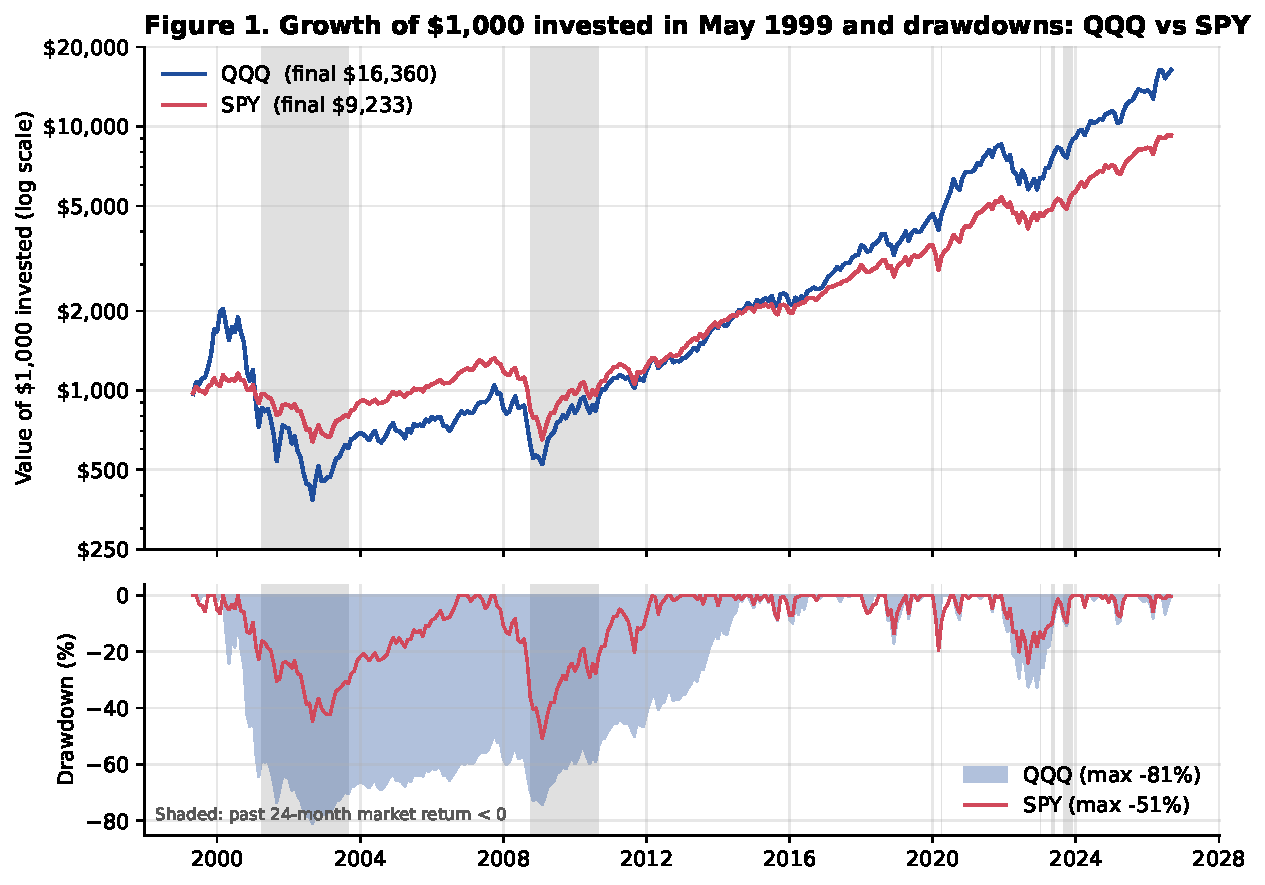
\includegraphics[width=0.9\linewidth]{graphic1_growth_drawdown.pdf}\end{figure}
\what Top: value of \$1,000 invested in May 1999, $W_t=1000\prod_{s\le t}(1+R_s)$, on a log scale.
Bottom: drawdown, $DD_t=W_t/\max_{s\le t}W_s-1$, the loss from the previous peak.

\find Final value: QQQ \$16,360 vs SPY \$9,233. Maximum drawdown: QQQ $-81\%$ (trough Sep 2002, back to its old peak only in Oct 2014) vs SPY $-51\%$ (trough Feb 2009).

\mean QQQ ended with about 1.8 times the wealth of SPY, but its path was far rougher: an investor who bought at the 2000 peak waited 14 years to break even.
Higher return came together with much deeper losses.

\link Motivates the project: is QQQ's extra return a reward for skill or exposure (\emph{alpha}), or simply compensation for extra risk (\emph{factor risk})?

%-------------------------------------------------------------
\section*{Figure 2. Risk-return profile and rolling Sharpe ratio}
\begin{figure}[H]\centering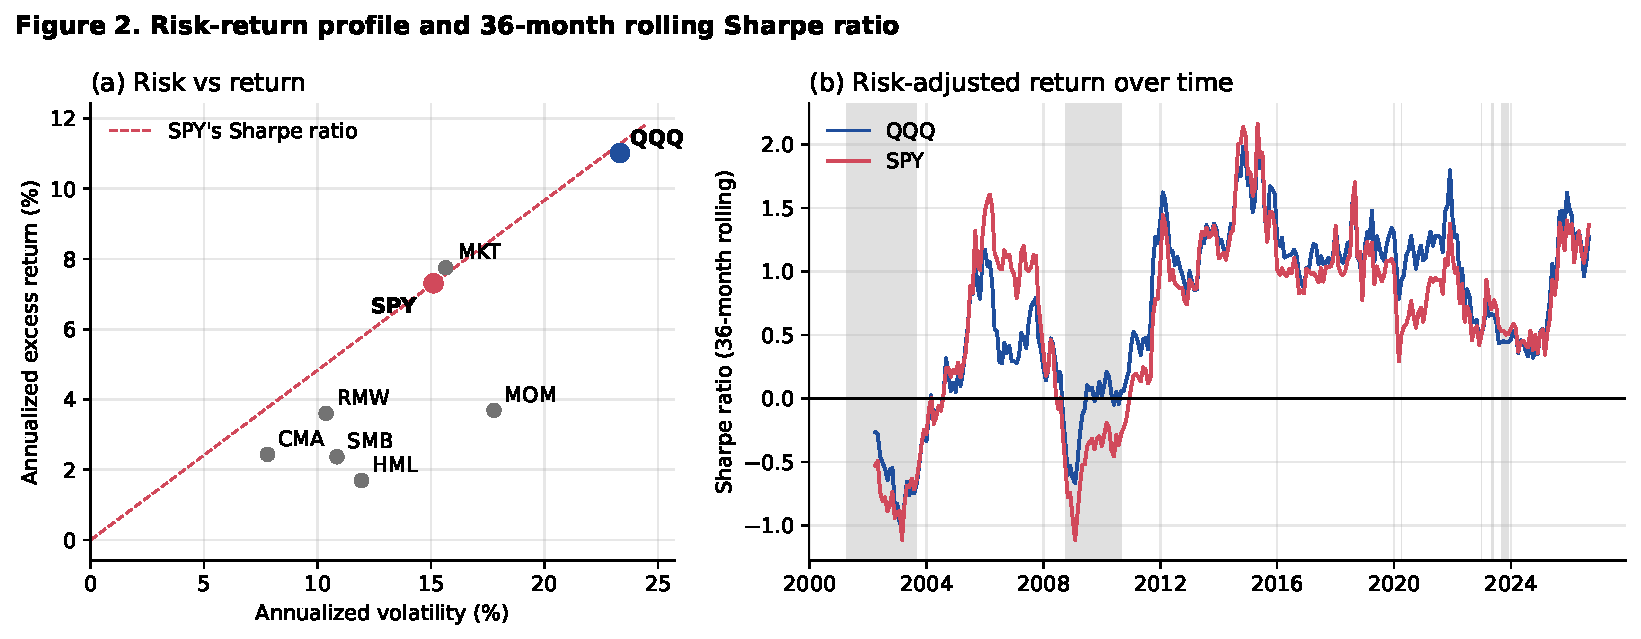
\includegraphics[width=0.95\linewidth]{graphic2_risk_return.pdf}\end{figure}
\what (a) Annualized mean excess return ($12\overline{EX}$) against annualized volatility ($\sqrt{12}\,s$) for QQQ, SPY and the six factors; the line from the origin through SPY has slope equal to SPY's Sharpe ratio.
(b) 36-month rolling Sharpe ratio, $SR_t=\sqrt{12}\,\overline{EX}_{t-35:t}/s_{t-35:t}$ \cite{sharpe66}.

\find QQQ: 11.0\% return, 23.3\% volatility; SPY: 7.3\% return, 15.1\% volatility. Full-sample Sharpe: QQQ 0.47 vs SPY 0.48.
QQQ was better on a risk-adjusted basis in 2009--2011 and 2020--2021; SPY was better in 2006--2007.

\mean QQQ sits almost exactly on SPY's Sharpe line: its higher average return is roughly what its higher volatility would predict.
Per unit of risk the two ETFs are nearly identical over the full sample; differences appear only in particular periods.

\link A first, informal answer to ``alpha or risk'': total volatility explains most of the premium. The regressions ask the sharper question of \emph{which} risks.

%-------------------------------------------------------------
\section*{Figure 3. Pairwise correlations}
\begin{figure}[H]\centering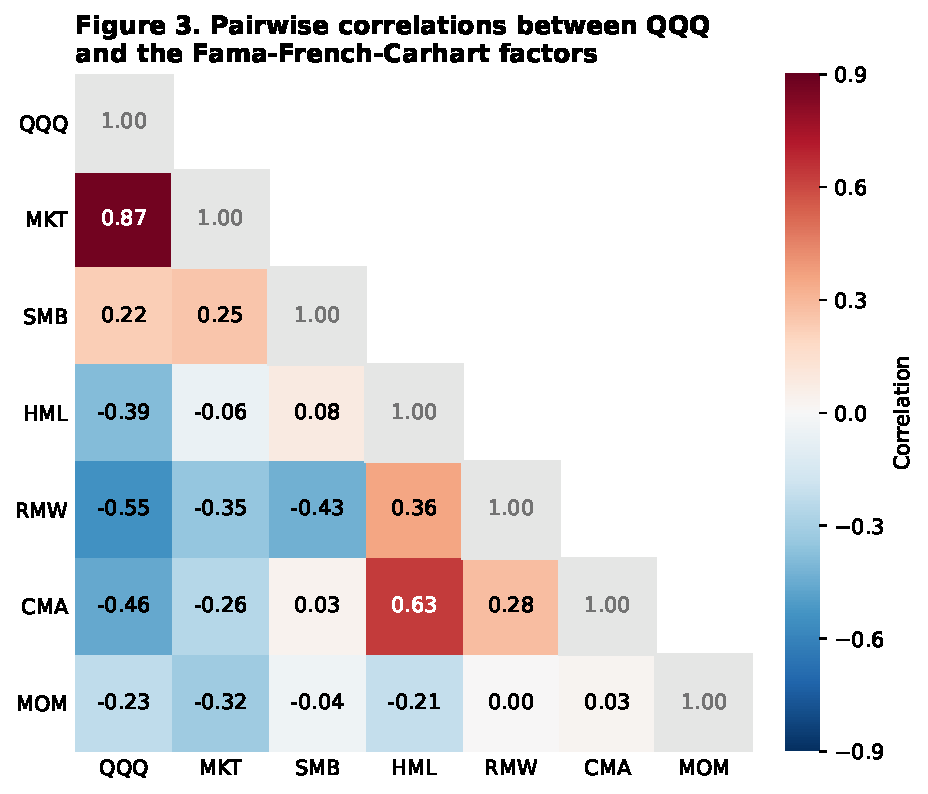
\includegraphics[width=0.6\linewidth]{graphic3_correlation.pdf}\end{figure}
\what Pearson correlations of $EX_{QQQ}$ and the six factors (lower triangle; red positive, blue negative).

\find $\text{corr}(EX_{QQQ},\text{MKT})=0.87$. QQQ is negatively correlated with RMW ($-0.55$), CMA ($-0.46$) and HML ($-0.39$).
Among the factors, $\text{corr}(\text{HML},\text{CMA})=0.63$ is the largest.

\mean The market explains most of QQQ's movement. The negative signs say QQQ behaves like growth stocks (anti-value), firms with weak current profitability relative to price, and heavy investors (anti-conservative).
The high HML--CMA correlation is a warning of multicollinearity: the two factors partly carry the same information, so their separate coefficients can be unstable \cite{ff15}.

\link Q2 (do RMW and CMA add information beyond FF3?) and the multicollinearity diagnostics (VIF, orthogonalization).
Q3 tests whether these exposures also explain the QQQ$-$SPY spread.

%-------------------------------------------------------------
\section*{Figure 4. Rolling alpha: CAPM vs five-factor model}
\begin{figure}[H]\centering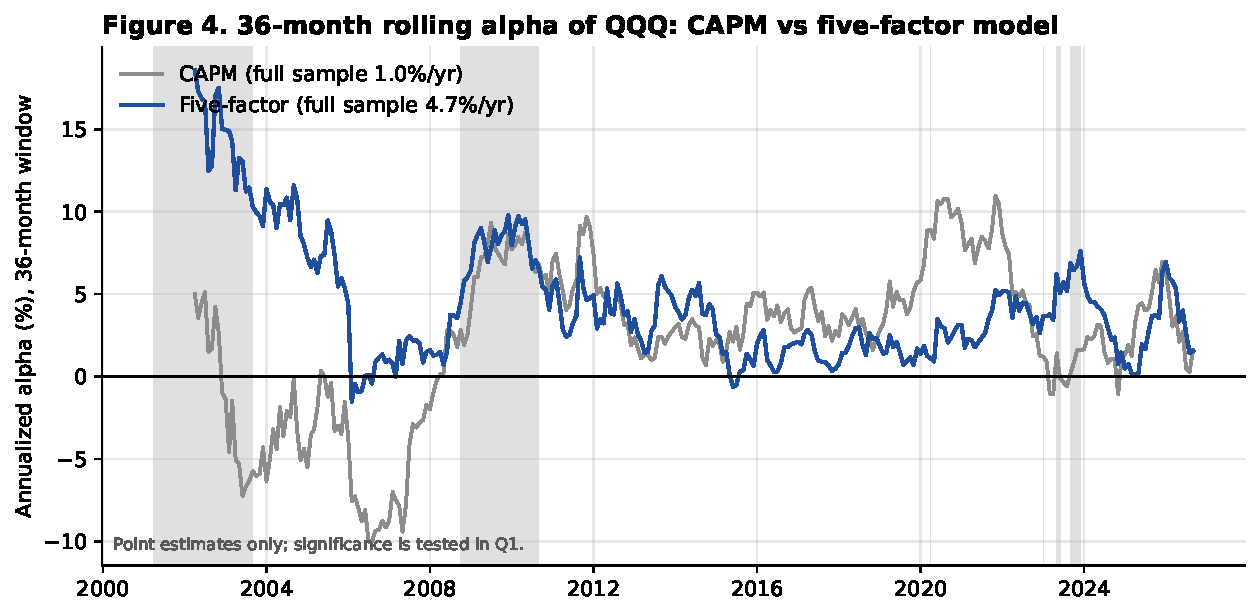
\includegraphics[width=0.9\linewidth]{graphic4_rolling_alpha.pdf}\end{figure}
\what For each month $t$, OLS on months $t-35,\dots,t$ of
\[
\text{CAPM: } EX_{QQQ}=\alpha+\beta\,\text{MKT}+\varepsilon,\qquad
\text{FF5: } EX_{QQQ}=\alpha+\textstyle\sum_{j}\beta_j F_j+\varepsilon,
\]
plotting the annualized intercept $12\hat\alpha$ \cite{jensen68}.
The intercept equals the average return left over after the factor-implied part: $\hat\alpha=\overline{EX}_{QQQ}-\sum_j\hat\beta_j\overline{F}_j$.

\find Full sample: CAPM $\hat\alpha=1.0\%$/yr, FF5 $\hat\alpha=4.7\%$/yr. Rolling CAPM alpha ranges from $-10\%$ (2006) to $+11\%$ (2021) and is positive in 77\% of windows; rolling FF5 alpha is positive in 97\% of windows, largest in 2002--2005 and 2009--2010.

\mean Against the market alone, QQQ shows little alpha. Adding factors makes alpha \emph{larger}, not smaller.
The reason is QQQ's negative loadings on HML, RMW and CMA, factors with positive average premia: the FF5 model says QQQ ``should'' have earned \emph{less} than the CAPM predicts, yet it did not.
These are point estimates only; whether $\alpha\neq0$ is tested in Q1 with Newey--West standard errors \cite{nw87}.

\link Q1: $H_0:\alpha=0$ in models M1--M4.

%-------------------------------------------------------------
\section*{Figure 5. QQQ vs market by bear-market state}
\begin{figure}[H]\centering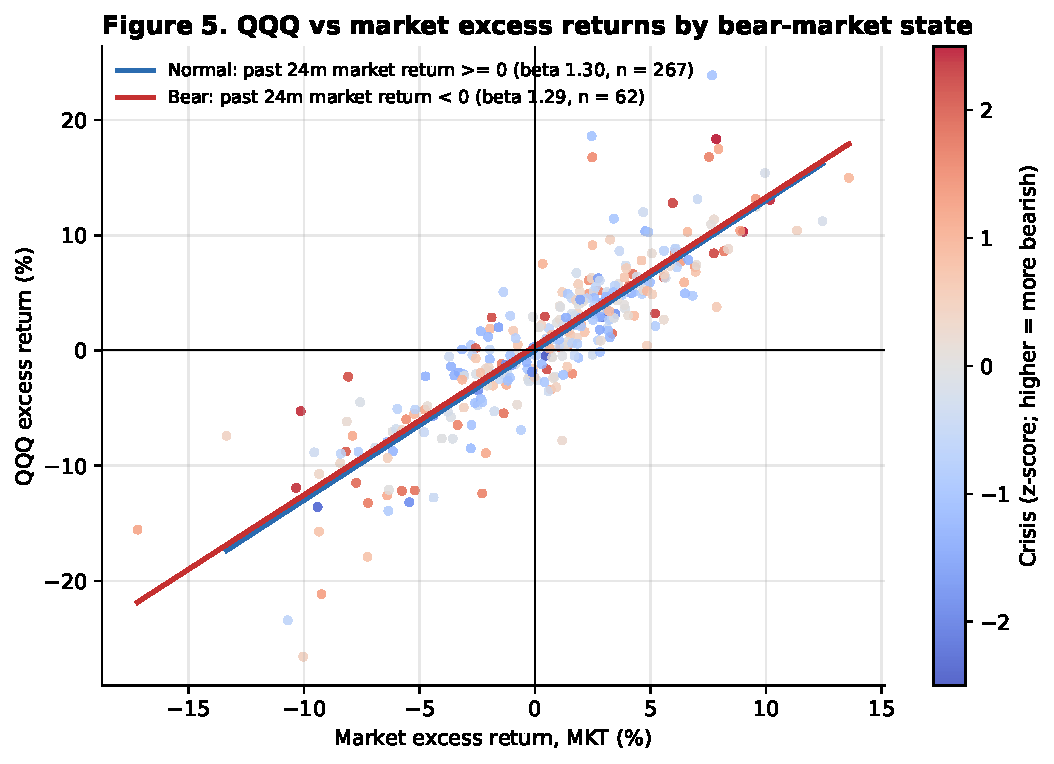
\includegraphics[width=0.75\linewidth]{graphic5_beta_by_state.pdf}\end{figure}
\what Each point is one month: $x=$ MKT, $y=EX_{QQQ}$, color $=$ Crisis, a continuous z-score $\text{Crisis}_t=-(\text{Past24}_t-\overline{\text{Past24}})/s_{\text{Past24}}$ (red = weaker past market).
Lines are OLS fits separately for normal ($\text{BEAR}=0$) and bear ($\text{BEAR}=1$) months.
The plot shows three variables at once (x, y, color).

\find Slope (market beta): normal months 1.30 ($n=267$), bear months 1.29 ($n=62$).

\mean QQQ moves about 1.3\% for every 1\% move in the market, and this sensitivity is essentially the same in bear and normal markets.
Bear-market months are more spread out (larger moves in both directions), but the slope does not steepen.
This differs from the strong state-dependence of momentum documented in \cite{dm16}.

\link Q4: $EX_{QQQ}=\alpha+\gamma\,\text{Crisis}+(\beta+\delta\,\text{Crisis})\,\text{MKT}_c+\dots$, testing $H_0:\delta=0$.
The figure suggests $\delta$ will be small and possibly insignificant.

%-------------------------------------------------------------
\begin{thebibliography}{9}\small
\bibitem{c97} Carhart, M. M. (1997). On persistence in mutual fund performance. \emph{Journal of Finance}, 52(1), 57--82.
\bibitem{dm16} Daniel, K., \& Moskowitz, T. J. (2016). Momentum crashes. \emph{Journal of Financial Economics}, 122(2), 221--247.
\bibitem{ff15} Fama, E. F., \& French, K. R. (2015). A five-factor asset pricing model. \emph{Journal of Financial Economics}, 116(1), 1--22.
\bibitem{jensen68} Jensen, M. C. (1968). The performance of mutual funds in the period 1945--1964. \emph{Journal of Finance}, 23(2), 389--416.
\bibitem{nw87} Newey, W. K., \& West, K. D. (1987). A simple, positive semi-definite, heteroskedasticity and autocorrelation consistent covariance matrix. \emph{Econometrica}, 55(3), 703--708.
\bibitem{sharpe66} Sharpe, W. F. (1966). Mutual fund performance. \emph{Journal of Business}, 39(1), 119--138.
\end{thebibliography}
\end{document}
